\documentclass{sig-alternate}

\usepackage{url} 
\usepackage{subfigure} 
\usepackage{color}
\usepackage{graphicx}
\usepackage{xspace}
\usepackage{listings}
\usepackage{enumerate} % easiest way to do roman numeral lists
\usepackage[usenames,dvipsnames]{xcolor} % more text colors!

\usepackage[font=footnotesize]{subfig}
\DeclareCaptionType{copyrightbox}
\hyphenation{op-tical net-works semi-conduc-tor}

\newif\ifdraft
%\drafttrue
\ifdraft
\newcommand{\tbnote}[1]{ {\textcolor{magenta} { ***TcB: #1 }}}
\newcommand{\jhanote}[1]{ {\textcolor{red} { ***SJ: #1 }}}
\newcommand{\mrnote}[1]{ {\textcolor{blue} { ***Melissa: #1 }}}
\newcommand{\egnote}[1]{ {\textcolor{green} { ***Emilio: #1 }}}
\newcommand{\hfnote}[1]{ {\textcolor{cyan} { ***HF: #1 }}}
\newcommand{\rajib}[1]{ {\textcolor{blue} { ***RM: #1 }}}
\newcommand{\brnote}[1]{ {\textcolor{Orange} { ***Brian: #1 }}}
\else
\newcommand{\rajib}[1]{}
\newcommand{\jhanote}[1]{}
%\newcommand{\note}[1]{ {\textcolor{blue} { ***NOTE: #1 }}}
\newcommand{\note}[1]{ {}}
\newcommand{\abhi}[1]{ {}}
\newcommand{\hfnote}[1]{}
\newcommand{\tbnote}[1]{ {}}
\newcommand{\brnote}[1]{ {}}
\newcommand{\egnote}[1]{ {}}
\fi

\newcommand{\pilotjob}{Pilot-Job\xspace}
\newcommand{\pilotjobs}{Pilot-Jobs\xspace}
\newcommand{\pilotdata}{Pilot-Data\xspace}
\newcommand{\pilotapi}{Pilot-API\xspace}
\newcommand{\bigjob}{BigJob\xspace}

\begin{document}

\conferenceinfo{XSEDE13}{'13 }
 \CopyrightYear{2013}

 \title{A Framework for Flexible and Scalable Replica-Exchange on
   Production Distributed CI}

\numberofauthors{5} 
\author{
\alignauthor
Melissa Romanus, Ole Weidner, Shantenu Jha \\
       \affaddr{Electrical and Computer Engineering, Rutgers University}\\
       \affaddr{Piscataway, NJ 08854}\\
       \email{shantenu.jha@rutgers.edu}
\alignauthor
Brian K. Radak,  Emilio Gallicchio, {Tai-Sung} Lee, Darrin M. York, Peng He, {Nan-Jie} Deng, Dai Wei, Ronald M. Levy\\
       \affaddr{BioMaPS Institute for Quantitative Biology and Department of Chemistry and Chemical Biology, Rutgers University}\\
       \affaddr{Piscataway, NJ 08854}\\
       \email{emilio@biomaps.rutgers.edu,\\york@biomaps.rutgers.edu,\\ronlevy@lutece.rutgers.edu}
}
\egnote{
\alignauthor
Melissa Romanus\\
       \affaddr{Electrical and Computer Engineering}\\
       \affaddr{Rutgers University}\\
       \affaddr{Piscataway, NJ 08854}\\
      \email{melissa.romanus@rutgers.edu}
\alignauthor
Emilio Gallicchio\\
       \affaddr{BioMaPS Institute for Quantitative Biology and Department of Chemistry and Chemical Biology, Rutgers University}\\
       \affaddr{Piscataway, NJ 08854}\\
      \email{emilio@biomaps.rutgers.edu}
\and  % use '\and' if you need 'another row' of author names
% 3rd. author
\alignauthor 
{Tai-Sung} Lee \\
       \affaddr{BioMaPS Institute for Quantitative Biology and Department of 
         Chemistry and Chemical Biology, Rutgers University}\\
       \affaddr{Piscataway, NJ 08854}\\
      \email{taisung@biomaps.rutgers.edu}
\alignauthor
Ole Weidner \
       \affaddr{Electrical and Computer Engineering}\\
       \affaddr{Rutgers University}\\
       \affaddr{Piscataway, NJ 08854}\\
      \email{ole.weidner@rutgers.edu}
\alignauthor 
Darrin M. York \\
       \affaddr{BioMaPS Institute for Quantitative Biology and Department of 
          Chemistry and Chemical Biology, Rutgers University}\\
       \affaddr{Piscataway, NJ 08854}\\
      \email{york@biomaps.rutgers.edu}
\and  % use '\and' if you need 'another row' of author names
% 3rd. author
\alignauthor 
{Nan-Jie} Deng \\
       \affaddr{BioMaPS Institute for Quantitative Biology and Department of 
         Chemistry and Chemical Biology, Rutgers University}\\
       \affaddr{Piscataway, NJ 08854}\\
      \email{nanjie.deng@gmail.com}
\alignauthor
Peng He \\
       \affaddr{BioMaPS Institute for Quantitative Biology and Department of 
         Chemistry and Chemical Biology, Rutgers University}\\
       \affaddr{Piscataway, NJ 08854}\\
      \email{hepeng.yanglu@gmail.com}
\alignauthor 
Dai Wei \\
       \affaddr{BioMaPS Institute for Quantitative Biology and Department of 
          Chemistry and Chemical Biology, Rutgers University}\\
       \affaddr{Piscataway, NJ 08854}\\
      \email{daiwei@physics.rutgers.edu}
\and
\alignauthor 
Ronald M. Levy \\
       \affaddr{BioMaPS Institute for Quantitative Biology and Department of Chemistry and Chemical Biology, Rutgers University}\\
       \affaddr{Piscataway, NJ 08854}\\
       \email{ronlevy@lutece.rutgers.edu}
\alignauthor 
Shantenu Jha \\
       \affaddr{Electrical and Computer Engineering, Rutgers University}\\
       \affaddr{Piscataway, NJ 08854}\\
       \email{shantenu.jha@rutgers.edu}
}

\maketitle

\begin{abstract}
  Replica-Exchange represent a powerful class of algorithms that are
  used for enhanced configurational and energetic sampling in a range
  of physical systems. Computationally they represent a type of
  applications with multiple scales of communication; at a
  fine-grained level there is often communication with a replica,
  typically an MPI process. At a coarse-grained level -- both
  temporally as well as in data amount exchanged, the replicas
  communicate with other replicas. In this paper, we outline a novel
  framework that we have developed that supports the large-scale and
  flexible execution of a number of replicas. The framework is
  flexible in the sense that it supports different coupling schemes
  between the replicas, and is agnostic to the specific underlying
  simulation -- classical or quantum, single-core simulation or a
  parallel simulation.  As a measure of the scalability of the
  framework, we measure the number of nanoseconds simulated a day, as
  a function of the number of replicas. In spite of the increasing
  communication and coordination requirements as a function of the
  number of replicas, our framework supports the execution of a
  thousand replicas without significant overhead. Furthermore, as
  representative of the efficiency of the framework, the number of
  nanoseconds simulated in twenty-four hours as a function of replicas
  remains essentially constant. Although there are several specific
  aspects that will benefit from further optimization, a first working
  prototype has the ability to fundamentally change the scale of
  replica-exchange simulations possible on production distributed
  cyberinfrastructure such as XSEDE, as well as support novel usage
  modes on these infrastructure. This paper also represents the
  release of the framework to the broader biophysical simulation
  community and provides details on its usage.
\end{abstract}





\category{H.4}{Information Systems Applications}{Miscellaneous}
%A category including the fourth, optional field follows...
\category{D.2.8}{Software Engineering}{Metrics}[complexity measures, performance measures]

\terms{Experience, Technology}

\keywords{HPC, Distributed Computing, IMPACT, AMBER, MD, Large Scale, XSEDE
  resources}

\section{Introduction}

\jhanote{ A description of the computational workflow, viz., the
  different
 machines/resources used, how many ensembles we
  simulated, data
 volumnes managed etc., (ii) any computational
  performance issues
 including (a) measuring "efficiency" as the
  number of distributed
 resources utilized goes as measured by $T_c$
  (time to completion),
 (b) $T_c$ as a function of the number of
  replicas, and (iii) a
 description of the software infrastructure
  that is employed to
 enable distributed replica-exchange on XSEDE.}

\brnote{Some ideas via Darrin's comments:
 The infrastructure
  described herein is immediately applicable to several
 important
  problems, including, but not limited to, probing the chemical
  mechanisms of enzymes via quantum mechanical/molecular mechanical 
  simulations. While such an approach has long been considered as
  ideal, it has
 not widely been used due to difficulties in its
  efficient implementation. The
 work here presents the immediate
  possibility of its routine application
 across multiple software
  and hardware architectures.}


\jhanote{A description of the computational workflow, viz., the
  different machines/resources used, how many ensembles we simulated,
  data volumnes managed etc., (ii) any computational performance
  issues including (a) measuring "efficiency" as the number of
  distributed resources utilized goes as measured by $T_c$ (time to
  completion), %(b) $T_c$ as a function of the number of replicas, and
  (iii) a description of the software infrastructure that is employed
  to enable distributed replica-exchange on XSEDE.}

\jhanote{Describe the need for large-scale simulations. Describe what
  is unique to replica-exchange. Challenges that arise from loose,
  intermittent (stochastic) coupling, as opposed to fixed exchanges}


\jhanote{(i) algorithmic advances coupled with infrastructural
  advances. (ii) the need for dynamic execution and resource
  management, (iii) which is why we believe pilot-jobs is a good
  abstraction (reference earlier work using BigJob). (iv) Novelty of
  this work is: (A) marriage of an application library for flexible
  replica-exchange simulations with scalable and dynamic resource
  management, (B) demonstration of a framework for different and
  tunable replica coupling schemes that can be used for QM and
  classical examples.}
 
\jhanote{Aim of this work is to present (i) the framework -- both
  components, (ii) understand and characterize basic performance}




Parallel Replica Exchange (RE)\cite{hansmann1999new,Felts:Harano:Gallicchio:Levy:2004,Andrec2005,Mitsutake2010} denotes a family of advanced
conformational sampling algorithms widely employed in molecular
simulations of chemical and biological systems. The key aspect of RE
algorithms is that multiple molecular dynamics (MD) threads (referred
to as “replicas”) each assigned to a different thermodynamic or
potential energy state of the system, are executed in parallel and, further,
replicas travel in configurational space as well as in state
space by communicating and stochastically exchanging their state
assignments with those of other replicas. Exchanges are controlled by
microscopic reversibility requirements ensuring that feasible
thermodynamic ensembles are sampled at each state.  It has been shown
in many contexts\cite{Woods2003,Murata2004,Bussi2006,Liu2006,Yeh2008,Meng2010,Gallicchio2011} that RE moves enhance
conformational mixing relative to multiplexed serial conformational
sampling algorithms based on teams of non-communicating
MD threads. Replica exchange algorithms indeed provide some of the
most powerful conformational sampling tools available, yielding
converged results orders of magnitude faster than
conventional approaches.

The advantages of RE approaches are however partly counterbalanced by
the additional complexities inherent in instating and maintaining a
communication framework among the MD threads. In practice this
requirement has historically discouraged large scale deployment of RE
on XSEDE. In our view this is not necessarily due to lack of suitable
hardware and networking resources, but rather to the lack of suitable
software technologies capable of efficiently harnessing this latent
computational power.

Although the coupling between replicas is conceptually simple and
relatively ``easy'', replica-exchange applications represent the
general challenge of scaling many loosely-coupled simulations. The
challenge arises from the fact that although most communication is
internal to the individual replicas which are large-scale MPI-style
simulations, there exist a less frequent but often a slow
communication mode which increases in complexity, importance and cost
as the number of replicas increases. Providing an approach that works
across multiple replica sizes, replica numbers and coupling schemes
both a software and conceptual challenge. The state of replicas is typically changing and they often change
depending upon the outcome of the an exchange. Furthermore, resource
assignment and scheduling is typically required after an exchange.
Thus there is a need for finer grained resource management than is
typically provided by the batch-queue level resource management. 

To address some of these issues, there has been recent progress
towards  asynchronous RE formulations based on a pilot-job framework, that can support
dynamic and scalable resource execution and management, and thereby
provides the basis for a flexible and scalable formulation of
replica-exchange on XSEDE. These developments are the subject of this report.


Many applications areas, such as the ones illustrated here,
benefit greatly from multi-dimensional RE implementations employing
hundreds to thousands of replicas. However, current implementations
of the replica exchange method in use by the computational chemistry
community are severely limited in terms of it scalability and control
when many replicas are involved. In conventional implementations of
RE\cite{Jiang_JChemTheoryComput_2012_v8_p4672},\brnote{2012 JCTC paper describing synchronous RE on BlueGene/P} 
simulations progress in unison and exchanges occur in a
synchronous manner whereby all replicas must reach a pre-determined
state (typically the completion of a certain number of MD steps),
before exchanges are performed. This synchronous approach has a number
of severe limitations. Firstly, sufficient dedicated computational
resources must be secured for all of the replicas before the
simulation can begin execution. Secondly, the computational resources
must be statically maintained until the simulation is
completed. Thirdly, failure of any replica simulation typically causes
the whole calculation to abort. The reliance on a static pool of
computational resources and zero fault tolerance prevents the
synchronous RE approach from being a feasible solution for large scale
RE deployments.

As earlier prototypical implementations of asynchronous RE (aRE)
algorithms\cite{Gallicchio2008} have illustrated, the replica
exchange method itself does not impose the restriction that exchanges
should occur synchronously across all threads and that all of the MD
threads should run at the same time. The basic idea of asynchronous
RE is to allow pairs of replicas to perform exchanges independently
from the other replicas. This paradigm lends itself naturally to
implementations based on the pilot-job framework described below,
which, while already extensively employed to automate the asynchronous
execution of independent ensembles, as shown in this work, can be
effectively employed to manage inter-communicating MD threads.

In this work we present ASyncRE, an asynchronous RE software utility
deployed built on the BigJob/SAGA distributed computing environment on
XSEDE capable of scaling to arbitrarily large numbers of
replicas. Illustrative applications of the software to large-scale
multi-dimensional RE problems are presented and analyzed.

\section{Scientific Problem}\label{sec:requirements}

The conformational sampling problem in molecular simulations can be described 
as the problem of efficiently drawing samples $x$ from the canonical 
distribution of the chemical system:
\begin{equation}
p(x;\beta,\theta) = \frac{\exp[-U(x;\beta,\theta)]}{Z} \, ,
\end{equation}
where $x$ represents the configuration of the system (atomic coordinates), $Z$ 
denotes the configurational partition function, $\beta=1/k_B T$ is the inverse 
(absolute) temperature, and $U(x;\beta,\theta)=\beta V(x;\theta)$ is the 
dimensionless potential energy of the system.  $U(x;\beta,\theta)$ depends 
linearly on the inverse temperature and on the potential energy parameters 
({\em e.g.} the atomic charges or parameters of any biasing potentials), 
collectively denoted as $\theta$ (more generally, $U(x;\beta,\theta)$ also 
depends on the applied pressure or component chemical potentials when using 
the isobaric or (semi-)grand canonical ensembles, respectively).

In conventional MD-based sampling implementations, $x$ evolves in time with 
fixed model parameters. Slow convergence is the main issue of concern with 
methods of this kind as it is notoriously difficult to achieve equilibration 
within the time scale afforded by even the fastest supercomputers. Fortunately,
great progress has been achieved in recent years with the development of 
generalized ensemble formulations, which now allow modeling of complex 
biochemical processes with unprecedented fidelity. This sampling enhancement is
achieved via a random walk, not only in conformational space, but also in 
parameter space.

Amongst generalized ensemble sampling algorithms, replica exchange molecular
dynamics (REMD) remains one of the most convenient and effective due to its 
broad applicability and amenability to nearly all parallel computing 
architectures. The core concept of REMD is that multiple replicas traveling in
conformational space are additionally enabled to move in parameter space by 
exchanging state parameters amongst each other. The first and most widely 
employed RE scheme is temperature REMD (T-REMD) in which inverse temperatures 
$\beta_i$ are exchanged. T-REMD accelerates interconversions between stable 
states of the system by letting replicas temporarily visit high temperatures 
where barrier crossings are more rapid. However, REMD schemes can involve 
exchanges of any number of state parameters. For example, schemes involving the
exchange of more than one parameter are often referred to as 
\emph{multi-dimensional} REMD schemes.\cite{Mitsutake2010}

Any REMD scheme is required to satisfy microscopic reversibility. In the 
present context this is ensured by structuring exchanges so that permutations 
of state parameters assigned to replicas are distributed according to the 
discrete unnormalized probability distribution:\cite{chodera2011replica}
\begin{equation}
p(\{j_M\})=\exp\left[-\sum_{i=1}^M U(x_i;\beta_{j_i};\theta_{j_i})\right] \,
\end{equation}
where $\{j_M\}$ denotes one of the $M!$ permutations of a vector of $M$ states,
$x_i$ is the atomic configuration of replica $i$, and $\beta_{j_i}$ and 
$\theta_{j_i}$ are the inverse temperature and potential parameters assigned to
replica $i$.

In this work we analyze four science application areas that benefit from the 
application of multi-dimensional REMD protocols. The first is the modeling of 
binding between a guest molecule (cyclooctanol) and a host 
($\beta$-cyclodextrin) to form a supramolecular complex in solution.\cite{Gallicchio2012a} In this case the dimensionless energy is:\cite{Gallicchio2010}
\begin{equation}
U(x;\beta,\lambda) = \beta V_0(x) + \beta \lambda u(x) \,
\end{equation}
where $V_0(x)$ is the potential energy when the host and the guest are 
separated, $u(x)$ is the interaction energy between the host and the guest, and
$\lambda$ is an alchemical parameter ranging between 0 and 1. This systems is 
modeled by multi-dimensional RE with up to 192 \egnote{modify as needed} 
replicas corresponding to all possible combinations of 8 temperatures 
distributed between 300 and 600K and 24 $\lambda$'s ranging between 0 and 1. 
The purpose of the sampling along $\lambda$ is to enhance mixing of 
conformations along the alchemical pathway while high temperatures enhance 
sampling at each alchemical stage.

The second application studied by multi-dimensional RE is the folding of the 
TrpCage mini-protein. In this case the dimensionless potential energy function 
is
\begin{equation}
U(x;\beta,\lambda) = \beta V(x) + \beta w_{\rm Go} V_{\rm Go}(x) \,
\end{equation}
where $V(x)$ is the unbiased potential energy, $V_{\rm Go}$ is a biasing 
potential favoring the formation of natively folded conformations,\cite{pogorelov2004variations} and 
$w_{\rm Go}$ is an energy weight ranging between 0 (no bias) to $0.42$ in this 
case (maximal bias). This system is studied with up to 336 \egnote{modify as 
  needed} replicas corresponding to all possible combinations of 24 
temperatures between 300 and 600K and 14 values of  $w_{\rm Go}$ between 0 and 
$0.42$. The purpose of this protocol is to bias the system so as to enhance the
rate of folding and unfolding at multiple temperatures.

The last two applications employ multi-dimensional replica exchange umbrella 
sampling (RE-US), but in two quite different scenarios, thus demonstrating the 
broad applicability of the approach.  In all RE-US simulations, the 
dimensionless potential energy can be written as
\begin{equation}
U(x;\beta,\lambda) = \beta V_0(x) + \beta \sum_{n=1}^N W_n(x_n)
\end{equation}
where $V_0(x)$ is the unbiased potential and $W_n(x_n)$ is a bias potential 
applied to the $n$th bias coordinate in order to localize sampling to high 
energy regions of configuration space that might not otherwise be sampled. For 
convenience (as is typical) we choose $W_n(x_n)$ to have a harmonic form. 

In the first RE-US scheme, the well-known alanine dipeptide model for protein 
the backbone is examined, and conformational biases are applied to the 
$\phi$/$\psi$ torsion angles. The complete range of 360 degrees is divided into
15 degree intervals for both angles, resulting in 576 replicas. Although this 
is a common test case for enhanced sampling protocols, we increase the demand 
here by treating the solvent bath explicitly. The second application is a 
phosphoryl transfer reaction in solution, a prototype reaction for multiple 
protein and ribonucleic acid enzymes. Biases are applied to the breaking and
forming bonds. The chemically reactive solute is treated quantum mechanically, 
whereas the solute is treated by classical molecular mechanics. 

Due to numerous calculations needed in quantum calculations and the unfavorable
scaling of these calculations (unlike classical force fields, quantum 
potentials cannot be described as pair-wise interactions), it is extremely 
difficult to sample over the conformational space to obtain sufficient and 
meaningful ensembles.  Hence the advantages of a RE-US approach are especially 
important in QM simulations, such as the example system presented here.  RE-US
is one of the most promising ways to increase the feasible application of 
quantum potentials via increased sampling efficiency.

\subsection{Computational Requirements}

As introduced above and further elaborated below, in order to
efficiently perform large scale RE calculations of this kind on XSEDE
we adopt an asynchronous formulation of RE, which, unlike conventional
synchronous implementations, requires only a fraction of the computing
resources nominally required by the application [(number of replicas)
  times (number of CPU cores per replica)]. Furthermore the loss of
computing resources does not cause termination of the
application. Conversely, it allows the expansion of the application
dynamically as new resources become available.

In the current implementation, communication between pairs of replicas
is achieved through a shared filesystem while they are temporarily
checkpointed and not actively running. This approach has the advantage
of being very general and well supported by BigJob. It also does not
require source code modification of legacy MD kernels.

\section{Software Environment}

XSEDE is inherently a complex infrastructure with heterogeneous
resources. In order to harness the power of such a distributed
environment, we utilize Pilot-Jobs. A Pilot-Job is a mechanism by 
which a proxy for the actual simulations
is submitted on the resource to be utilized; this proxy agent in turn,
is given responsibility to convey to the application the availabilty
of resources and also influence which tasks are executed. The
abstraction of a Pilot-Job generalizes the reoccurring concept of
utilizing a placeholder job as a container for a set of compute tasks;
instances of that placeholder job are commonly referred to as
Pilot-Jobs or pilots. 

In general, Pilot-Abstractions provide a suitable means to marshal
heterogeneous sets of both compute and data resources and support the
efficient utilization of different kinds of commercial as well science
cloud resources. Pilot-Abstractions have been extensively used on both
HPC and HTC infrastructures for a range of application scenarios as a
resource management abstraction to, (i) improve the utilization of
resources, (ii) to reduce wait times of a collection of tasks, (iii)
to facilitate bulk or high-throughput simulations where multiple jobs
need to be submitted which would otherwise saturate the queuing
system, and (iv) as a basis to implement application specific
execution, scheduling and policy decisions

The P* model~\cite{pstar12}, a model for Pilot-Abstractions, worked to clearly
define the computation and data components of a distributed
application as 'compute units' and 'data units' in the context of
Pilot-Jobs and Pilot-Data. A compute unit describes a self-containing
piece of work, e.g. a computational task that potentially operates on
a set of input data, while a data unit is a container for a logical
group of data that is often accessed together or comprises a larger
set of data; e.g. a data file or chunk.


\subsection{BigJob: A Pilot-based Framework}

%A specific implementation of the P* model is 
BigJob is a pilot-job system implementation which provides a framework
for running many types of distributed applications -- including but
not limited to very-large scale parallel simulations, many small
high-throughput simulations, or ensemble-based workflows. Consistent
with the P* model, BigJob (BJ) provides a unified runtime
environment for Pilot-Jobs on heterogeneous
infrastructures. For this purpose, BigJob provides a higher-level,
unifying interface to heterogeneous and/or distributed data and
compute resources. The framework is accessed via the Pilot-API, which
provides two key abstractions: Pilot-Job and Pilot-Data.

Applications can specify their resource requirements using a Pilot
description. In the compute case, the user typically specifies the
application to run as well as the number of cores required by their
application.  Pilots are started via the Pilot-Compute Service. BigJob 
eliminates the need to interact with different kinds of compute
resources, e. g. batch-style HPC/HTC resources as well as cloud
resources, and provides a unified abstraction for allocating
resources. 

BigJob has seen its widest usage across the heterogeneous resources
that XSEDE provides. Simple installation into user space on any
resource that supports Python 2.5 or greater makes the uptake of
BigJob easy for the end user. BigJob supports thousands of jobs and
millions of SUs on XSEDE. It has been at the heart of two recent and
successful ECSS projects.

% BigJob has historically been used for parameter sweeps, many instances
% of the same task (ensemble), chained tasks, loosely coupled but
% distinct tasks, as well as tasks with data or compute dependencies.

\subsection{SAGA: Interoperability Layer}

In order for BigJob to work on heterogeneous resources, it requires an
interoperability layer which provides access to a variety of
middleware.  This is achieved through the use of The Simple API for Grid Applications (SAGA).
SAGA defines a 
high-level access mechanism for distributed infrastructure components 
like job schedulers, file transfers, and resource provisioning services. 
Given the heterogeneity of distributed infrastructures, SAGA provides 
a much needed interoperability layer that lowers the complexity and 
improves the simplicity of using distributed infrastructure whilst 
enhancing the sustainability of distributed applications, services, and tools.

SAGA is an Open Grid Forum (OGF) recognized standard (GFD.90). 
It allows developers of distributed applications to construct
higher-level functionality and abstractions, such as
gateways, workflows, application management systems, and runtime
environments. The key advantages to running with SAGA on XSEDE
is that users do not need to worry about the individual batch
queueing systems implemented on the various machines. Using the 
SAGA API and appropriate job adaptors, the different submission
mechanisms for these queueing systems is handled on the SAGA backend,
which is transparent to the user.

The SAGA API has been used to provide almost complete
coverage over nearly all grid and distributed computing
middleware/systems, including but not limited to Condor, Genesis,
Globus, UNICORE, SGE, LSF/PBS/Torque, and Amazon EC2.

\subsection{Deployment of BigJob}

SAGA and BigJob are lightweight enough that they can be easily installed into
the home directory of a user using the Python Package Index
(PyPi). SAGA is packaged within BigJob, so users do not have to worry
about installing two separate modules.

Since the main deployment is on XSEDE, we do not recommend altering
the default PYTHONPATH of the machines. Instead, we encourage users to
use a virtual environment. A virtual environment allows a user to
create a local Python software repository in his or her home directory
that behaves exactly like the global Python repository, except that it
grants the user \textit{write} access to it. In order to use the virtual
environment, the Python version must be greater than 2.4. Since some
XSEDE machines use Python 2.4 as the default python version, it may be
required to load a python module file before installing BigJob.

After activating the virtual environment, the BigJob python package
can be installed by typing:

\begin{lstlisting}[frame=single]
easy_install bigjob
\end{lstlisting}

In addition to the BigJob package, the BigJob python
dependencies, including the SAGA package, are also installed. 
The SAGA package includes
the proper adaptors for a wide variety of middleware systems. This
allows the user to submit jobs to any of the XSEDE batch
queuing systems.

BigJob requires SSH password-less login to the machines and a redis
server running either locally or on a remote server. The redis server
is used for coordination of the pilot-job and its compute and data
units. For the purposes of this project, we utilize a private redis
server hosted on a virtual machine at Indiana University. In order to
provide a more seamless uptake of BigJob by users, we will provide an
open-access redis server available on XSEDE. This avoids the overhead
of new users having to start a redis-server on an XSEDE machine's head
node or on their local machines. This effort is currently underway
with XSEDE ECSS staff to make the server only accessible to registered
users of XSEDE.

After following the aforementioned steps, users will be able to write
their own BigJob submission scripts using Python. These scripts can
range from simple ensemble-based simulations to more complicated
workflows based on the users' needs.

\subsection{Async Replica-Exchange}

ASyncRE is a Python package to perform file-based asynchronous
parallel replica exchange molecular simulations. The current
implementation is aimed at computer clusters managed by a queuing
system and supported by a shared filesystem. The BigJob distributed
computing infrastructure is used for job launching and monitoring.

The ASyncRE package includes a core module which performs common tasks
such as job staging through BigJob and exchanging of parameters among
replicas. Support for arbitrary MD engines and RE schemes are
introduced through user-provided modules (Figure \ref{fig:aRE_chart}). Currently, MD
engine modules are available for the AMBER and IMPACT MD programs. A
similar modular mechanism provides support for arbitrary RE schemes
(temperature, Hamiltonian, etc.), including arbitrary multidimensional
combinations of these (such as 2D RE temperature/Hamiltonian). The
software is currently distributed with modules for multi-dimensional RE
umbrella sampling with AMBER\cite{AMBER12}, and BEDAM $\lambda$-RE alchemical binding
free energy calculations with the IMPACT MD engine \egnote{[BEDAM papers]}.

The BigJob-based Asynchronous Replica-Exchange based framework is (ASyncRE) is available for public download at: \\
\url{https://github.com/saga-project/asyncre-bigjob}

\begin{figure}
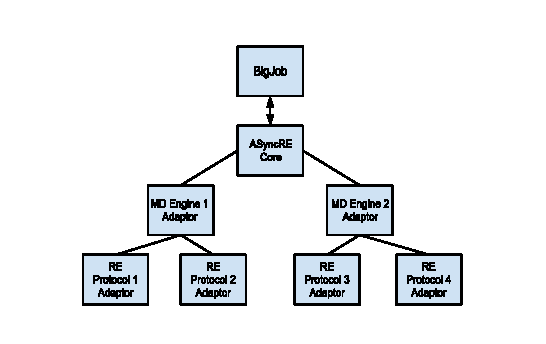
\includegraphics[width=3in]{asyncre.eps}
\caption{\label{fig:aRE_chart}The structure of the ASyncRE
  library. The ASyncRE Core module implements all of the
  general-purpose facilities to start and monitor replicas via BigJob,
  and coordinates replica exchanges. Routines implemented in adaptor
  modules perform functions specific to particular combinations of MD
  engines and RE schemes such as AMBER+umbrella sampling or IMPACT+BEDAM.  }
\end{figure}


The algorithm implemented by ASyncRE can be summarized as follows:

\begin{enumerate}

\item Job files and executables for the replicas are set up as
  appropriate for the MD engine/RE scheme combination as specified by
  the user-provided module/script. Typically this is accomplished by parsing a
  set of template input files according to the thermodynamic and
  potential energy settings which distinguish one replica from
  another. Each replica lives in a separate sub-directory of the
  working directory. These replica sub-directories are named
  \verb+r0+, {\tt r1}, $\ldots$,\verb+r<M-1>+, where \verb+M+ is the
  number of replicas.

\item Periodically, a randomly chosen subset of the replicas are
  submitted to BigJob for execution and enter a "R" (running)
  state. When a replica completes a run (of length specified in the MD
  engine input file), referred to in what follows as a "cycle", it
  enters a "W" (waiting) state which makes it eligible for exchange of
  thermodynamic and other parameters with other replicas and for the
  initiation of a new run cycle.

\item Periodically, exchanges of thermodynamic parameters are
  performed between the replicas in the waiting state based on the
  appropriate replica exchange rules (as specified in user modules)
  based on their thermodynamic states (temperature for example), or
  potential energy settings, together with the necessary structural
  and energetic information obtained from the MD engine output files.

\end{enumerate}

Internally a dictionary named \verb+status+ is used to keep track of
the status of the replicas (the current cycle, thermodynamic state,
running status, etc.) The status of the application is check-pointed
periodically using pickle. When restarting a previously stopped job,
the 'status' data structure is restored from this file and the
calculation proceeds from where it was left off.

An important feature of ASyncRE is the use of a ``run buffer'' to hide
latencies involved in the management of replica exchanges. Basically,
ASyncRE submits subjobs to BigJob in excess of the compute resources
allocated.  The result is that the submission of a replica
to BigJob for execution in general does not imply immediate execution;
rather, the replica is packaged in a BigJob compute unit which is
ready to begin execution as soon as BigJob can gather sufficient CPU
resources for it. In this way BigJob does not have to wait for a
replica to be prepared for a run cycle before it can execute it;
replicas are launched from a pool of replicas already prepped for
execution.

\subsubsection{AsyncRE Installation}

Following the installation of BigJob (see above) in the virtual user Python environment, ASyncRE is installed using PyPi as follows:

\begin{lstlisting}[frame=single]
pip install numpy
pip install configobj
pip install async_re-0.1.0.tar.gz
\end{lstlisting}

\verb+numpy+ and \verb+configobj+ are currently required dependencies
that will be installed automatically after the ASyncRE software will
be integrated into the PyPi archive. \\ \verb+async_re-0.1.0.tar.gz+ is
the current Python distribution package for ASyncRE. The library will
be soon made available publicly through \verb+github+.

In addition to installing the package in the virtual environment, it
is convenient to maintain a copy of the ASyncRE modules, scripts, and
examples in an easy-to-access location, such as:

\begin{lstlisting}[frame=single]
cd ~/src
tar zxvf async_re-0.1.0.tar.gz
\end{lstlisting}

Current application-level class files (such as
\\ \verb+amberus_async_re.py+ behave as executable scripts when launched
directly (see below). Documentation files can be found in the
\verb+doc+ subdirectory and sample files in the \verb+examples+
subdirectory of the package directory.

\subsubsection{ASyncRE Execution}

A typical sequence of commands to initiate an ASyncRE run on XSEDE is as follows:

\begin{lstlisting}[frame=single]
ssh <cluster_head_node>
source ~/.bigjob/bin/activate
cd <working_directory>
python amber_us.py control_file.cntl\
 > LOG 2>& &
\end{lstlisting}

The second command above activates the virtualenv Python environment (see above). \verb+amber_us.py+ is a simple user-provided python script that loads the appropriate modules and launches the asynchronous RE simulation. For example for AMBER/umbrella sampling it is:

\begin{lstlisting}[frame=single]
import sys
from amberus_async_re \
 import amberus_async_re_job
# Parse control file
usage = "%prog <ConfigFile>"
if len(sys.argv) != 2:
    print "Please specify ONE input file"
    sys.exit(1)    
commandFile = sys.argv[1]
# initializes asynchronus RE simulation
rx = amberus_async_re_job\
 (commandFile, options=None)
rx.setupJob()
# starts submitting replicas to BigJob
rx.scheduleJobs()
\end{lstlisting}

A control file (\verb+control_file.cntl+ above) containing keyword/value pairs is used for setting ASyncRE runtime parameters. An example of a control file for AMBER umbrella sampling simulations is:

\begin{lstlisting}[frame=single]
#-Main settings------------------------
ENGINE = 'AMBER'
RE_TYPE = 'AMBERUS'
RE_SETUP = 'yes'
VERBOSE="yes"
ENGINE_INPUT_BASENAME = 'DMP_US'
ENGINE_INPUT_EXTFILES =\
 'DMP_US.parm7,DMP_US_0.rst7'
#-RE/simulation settings---------------
FORCE_CONSTANTS = \
'5.0,5.0:5.0,5.0:5.0,5.0:5.0,5.0'
BIAS_POSITIONS = \
'275.,275.:275.,280.:280.,285.:285.,280'
#-BigJob settings----------------------
WALL_TIME=200
COORDINATION_URL="redis://<redis_server>"
RESOURCE_URL="pbs://localhost"
QUEUE="batch"
BJ_WORKING_DIR='/home/user/amber_us/agent'
TOTAL_CORES=16
SUBJOB_CORES=8
#---------------------------------------
\end{lstlisting}

A detailed description of these settings is provided in the ASyncRE user documentation.


The command above causes, among other things, the submission of a job
to the local queuing system named \verb+bliss_job+. Execution terminates after a specified amount of
wall-clock time. The internal state of the simulation is check-pointed
periodically and at the end of execution so that it can be restarted
at a later time. Failed runs are automatically detected
and the relevant replicas are reset and restarted.

The ASyncRE package is users-extensible. Users are free to implement
RE modalities not natively supported by the current ASyncRE package
(see details on writing extension modules in the ASyncRE
documentation). Scripts that implement user-provided RE schemes are
typically preceded by customized classes/methods (usually overrides of
ones inherited from the main class). An example of a custom script application is:

\begin{lstlisting}[frame=single]
import sys, math, os, ...
from amber_async_re import pj_amber_job

class myREscheme_async_re_job(pj_amber_job):
    def _checkInput(self):
       ...
    def _buildInpFile(self, replica):
       ...
    def ...
    ...

if __name__ == '__main__':
   # Parse control file
   usage = "%prog <ConfigFile>"
   if len(sys.argv) != 2:
      print "Please specify ONE input file"
      sys.exit(1)    
   commandFile = sys.argv[1]
   # initializes asynchronus RE simulation
   rx = myREscheme_async_re_job\
(commandFile, options=None)
   rx.setupJob()
   # starts submitting replicas to BigJob
   rx.scheduleJobs()
\end{lstlisting}

\section{Large-Scale Replica Exchange on XSEDE: Experiments and
  Results}\label{sec:results}

\subsection{Performance Model}

Like many complex distributed applications, replica exchange consists of
multiple individually developed components that are combined and orchestrated to
carry out the application workload. In our implementation of the replica
exchange workflow, we identify three distinct  components: (1) BigJob as the
underlying PilotJob system, (2) ASyncRE as  the replica exchange application
framework, and (3) AMBER / IMPACT as the  application kernels.

Each of the three component has its own performance characteristics and 
can introduce overhead to the overall application. We define overhead from an 
application perspective as the fraction of the application runtime that is 
not spent on running the application kernels, but on application management 
logic, communication and coordination.

From an application point of view, the most important performance metric 
is throughput, which is defined as nanoseconds of model simulation time 
achieved per hour compute time on a given number of CPU cores. This is 
equivalent with the time to completion ($TTC$) for a specific number of 
steps ($s$). On the lowest level, $TTC$ is the sum of the queue waiting time and 
the application runtime:

$$ TTC_s = T^{O}_Q + T_X $$

However, if the overall runtime of the simulation is sufficiently long, 
$T_Q$ becomes negligible. We split up $T_X$ into application 
kernel runtime $T_R$ and overhead. Since overhead can occur in all three
components, we define $T^{O}_{BJ}$ as the overhead introduced by BigJob,
$T^{O}_{RE}$ as the overhead introduced by the AsyncRE package, and 
$T^{O}_{K}$ as the overhead introduced in the application kernel itself:

$$ TTC_s = T_R + T^{O}_{BJ} + T^{O}_{RE} + T^{O}_{K}$$

Application kernel overhead occurs for example if the kernel supports 
thread-level parallelism but doesn't scale linearly with the number of 
threads. Overhead in ASyncRE occurs when the framework executes management 
tasks, e.g., finding matching exchange partners for a set of replicas and 
no computation happens during that time. Lastly, we consider BigJob 
overhead as the time that is spent by BigJob on the placement and monitoring 
of subjobs during which no computation occurs. This includes network
round-trip time for communication via Redis.

To measure the different aspects of application overhead, instrumentation 
of all three components is necessary. This is still work in progress and 
the experiments and results described below only implement probes on a 
very high level. Nevertheless, the model helps us to reason about the observed 
differences in application performance. Detailed measurements and 
instrumentation of BigJob and ASyncRE are planned for the future. 


\subsection{Systems Investigated} 

Four physical model systems were investigated, two each with the IMPACT and
AMBER MD engines. These systems represent broad classes of problems of chemical
interest, namely binding, ``large scale'' macromolecular folding, 
``small scale'' conformational changes, and chemical ({\em i.e.} bond 
breaking/forming) events. Briefly, the systems are as follows:\\
IMPACT (implicit solvent)
\begin{enumerate}
\item Host/guest binding of cyclooctanol/$\beta$-cyclodextrin. The exchange
  parameters are all permutations of the system temperatures and an
  alchemical parameter coupling the host/guest interactions.
\item Folding of the TrpCage mini-protein. The exchange parameters are all
  permutations of the system temperature and the coupling weight of a 
  Go-type biasing potential.
\end{enumerate} 
AMBER (explicit solvent)
\begin{enumerate}
\item Umbrella sampling of the backbone conformational space ({\i.e.} the 
  $\phi$/$\psi$ torsions) of alanine dipeptide. The exchange parameters are all
  permutations of harmonic biasing potentials on each torsion.
\item Hybrid quantum mechanical/molecular mechanical umbrella sampling of
  phosphoryl transfer in 2-hydroxy ethyl ethyl phosphate, a model reaction for 
  base catalyzed RNA cleavage. The exchange parameters are all permutations of 
  harmonic biasing potentials on the breaking and forming bonds.
\end{enumerate}

\subsection{Experimental Configuration}

Multiple RE simulations were performed on each system in one of three different
modes intended to probe various scaling aspects of ASyncRE and BigJob. All runs
were given a wall time of one hour (with appropriate extrapolations). The three
modes were as follows:
\begin{enumerate}[I]
\item (IMPACT systems 1-2, MM) Fixed Pilot size, fixed Pilot runtime, and varying number of replicas in proportion to the number of cores per replica
\item (AMBER system 1, MM-US) Fixed Pilot size and approximately fixed cycle
  length (in CPU time) while varying the number of concurrent jobs ({\em i.e.}
  the number of cores per job) and the simulation time of each cycle. 
\item (AMBER system 2, QM/MM-US) Fixed replica count (192) while varying the
  Pilot size % and the frequency of coordination?
\end{enumerate}

%$T_c = T_x + T_Q$ where terms are total time to completion, run time,
%time waiting in queue. we do not measure $T_W$. We  


\subsection{Results}


 Table \ref{table:impactSmall} reports the main results for the
cyclooctanol/$\beta$-cyclodextrin system. In this test the number of
replicas was varied from 768 to 192 by increasing the level of
parallelism of the IMPACT MD kernel (from 1 core per replica to 4),
while the size of the BigJob was kept fixed at 384 cores (half of the
CPU cores required to run all of the replicas at once). With 1 core
per replica and 768 replicas the measured throughput is 954 ns/day to
be compared with the nominal maximal throughput of $1,300$ ns/day
corresponding to uninterrupted MD at the measured MD CPU speed (4.2
minutes for 10ps per replica). The ratio of the observed throughput
over the maximum (73\%) measures the overhead imposed by replica
exchange coordination ($T^{O}_{BJ} + T^{O}_{RE}$ above).  We see that
the throughput (expressed in simulation time per day) is reduced from
945 ns/day with 768 replicas to 708 ns/day with 192 replicas. The
reduction is due in large part to parallelization overheads in going
from 1 core per replica, as it can be deduced from the time required
to complete one MD cycle (10,000 MD steps in this case). The parallel
efficiency is approximately 76 and 67\% with 2 and 4 cores,
respectively, which is reasonable for this very small chemical
system. The replica exchange coordination overhead remains
approximately constant; for the test with 192 replicas for example the
throughput is 76\% of the maximum similar to the 73\% measured with
768 replicas. This indicates that the ASyncRE+BigJob is capable of
handling this rather high replicas turn over (up to $4,000$ subjob
launches per hour) quite efficiently.




\begin{table}
\caption{\label{table:impactSmall}IMPACT I Small System, 384 Core BigJob, \\60 minute run time}
\begin{tabular}{| p{1.5cm} | p{1.7cm} | p{1.7cm} | p{1.7cm}|}
\hline
Number of Replicas & Cores/replica & time/cycle (min) & Throughput (ns/day) \\ \hline
768 & 1 & 4.2 & 945 \\ \hline
384 & 2 & 2.6 & 880 \\ \hline
192 & 4 & 1.5 & 708 \\ \hline
\end{tabular}
\end{table}

\begin{figure}
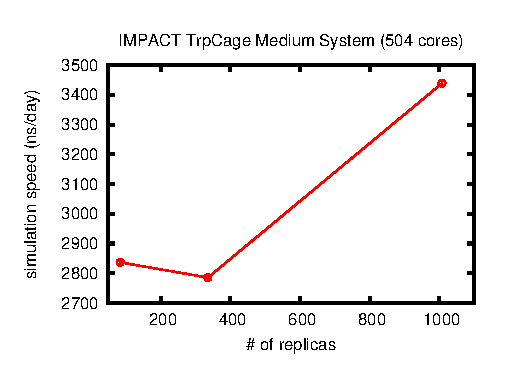
\includegraphics[width=3in]{impact_data/impact_trpcage.eps}
\caption{
  Scaling results for ASyncRE/BigJob for the folding of the TrpCage protein. Each run consisted of 504 cores divided amongst differing numbers of replicas. The maximum throughput is obtained 3.5$\mu$s/day with the largest number of replicas.
  \label{fig:impact_medium}
}
\end{figure}

The ASyncRE results for the folding of the TrpCage miniprotein (Fig. \ref{fig:impact_medium})  confirm the general trends observed for the smaller host-guest system above. For this case IMPACT's parallel efficiency is more favorable due to the greater number of atoms. It has been possible to test with the maximum number of cores per replica (12) allowed by the hardware. As expected maximum throughput (3.5$\mu$s/day) is obtained with serial replica execution with the largest number of replicas (1008). The maximum throughput in this case is 4.7 $\mu$s/day yielding a replica exchange overhead of 75\% similar to the host-guest system above. With the largest core count the throughput is 2.8 $\mu$s/day, lower than the observed maximum, but yielding a 6-fold speed up in terms of single-replica MD throughput. 

\begin{figure}
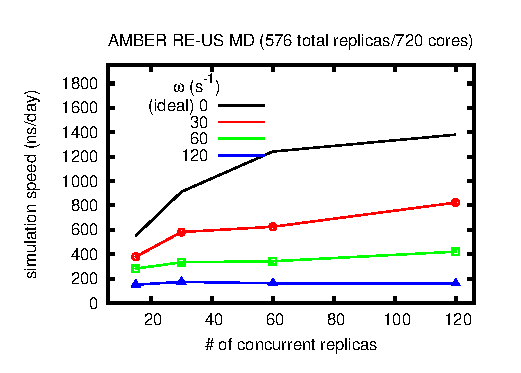
\includegraphics[width=3in]{amber_data/amber_mm.eps}
\caption{
  Scaling results for ASyncRE/BigJob with the AMBER MD engine employing a
  scalable molecular mechanics force field. Each run consisted of 720 cores
  divided amongst differing numbers of replicas (the pool of potential 
  replicas was fixed at 576) and coordination frequencies ($\omega$, {\em i.e.}
  the frequency with which simulations are started/stopped and exchanged). 
  Ideal performance (black line) would be obtained if there is no overhead in 
  launching or coordinating simulations ($\omega$ = 0). Increasing the 
  frequency with which replicas are ``launched'' results in diminished 
  performance, although the penalty for doing so appears to be fairly uniform 
  at higher frequncies (blue line).
  \label{fig:amber_mm}  
}
\end{figure}

Standard REMD simulations employing molecular mechanics (MM) force fields offer 
parallel scaling in both the number of replicas and the number of processors 
allocated to each replica. An optimal scheme would balance the efficiency gains
of both types of scaling in order to produce the most simulation time in real 
time. In order to assess the efficiency of ASyncRE/BigJob in combination 
with the AMBER MD engine, a fixed size pilot job of 720 cores was allocated 
(AMBER system 1 under Experimental Configuration) with various numbers of cores
allotted to each simulation. In this scheme, the number of simulations being 
coordinated in REMD varies, as well as the simulation rate (in ns/day) attained
by each replica. In order to probe the efficiency with which ASyncRE/BigJob 
coordinates simulations, the length of each simulation cycle (alternatively the 
frequency with which simulations are coordinated) was fixed in real time by 
varying the simulation time per cycle (Figure \ref{fig:amber_mm}). Ideal
performance would be obtained if there is no overhead in coordinating 
simulations. However, some cost must be incurred both in starting, stopping,
and restarting simulation cycles as well as in coordinating exchanges amongst 
stopped replicas, and the cost of this overhead is expected to increase as the 
frequency with which it is incurred increases. As seen in Figure 
\ref{fig:amber_mm}, this cost does indeed result in diminished output (as 
measured in ns/day) as the coordination frequency increases. However, for a
fixed coordination interval, the overhead appears to level out as a function
of the number of simulations being coordinated. This means that, at present, 
one can generally increase the number of replicas being simulated with only a
minor hit to performance.

Although in general one wants to produce as much simulation time as possible,
it is worthwhile to note that not all simulation time is equal, in the sense
that multiple short simulations do not usually contain as much statistical
information as a single short simulation. In fact, the basic aim of REMD is to
increase the statistical power of multiple simulations by facilitating the
exchange of information between them in a concerted fashion. This should be
kept in mind when analyzing performance graphs, as one might be tempted to run
as many small simulations as possible in an attempt maximize simulation speed.
For real applications and performance optimizations, other more physically and
statistically relevant metrics must be employed, but these are beyond the
scope of the present work.

\begin{figure}
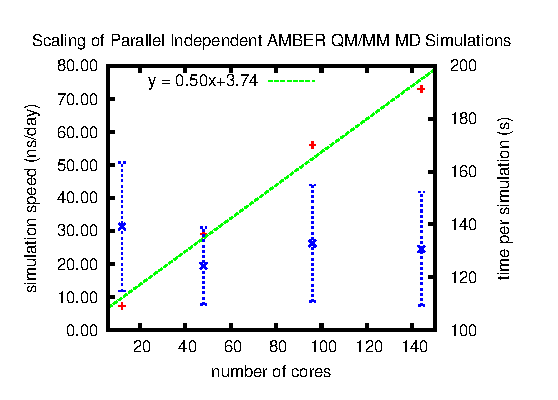
\includegraphics[width=3in]{amber_data/qmmm.eps}
\caption{
  Scaling results for ASyncRE/BigJob with the AMBER MD engine employing a
  serial quantum mechanical/molecular mechanical potential. The total number
  of cores allocated for the full REMD run was varied, while each simulation
  was run on a single core. As should be expected, performance (as measured in
  ns/day) increases linearly (red fit line) with the number of simulations 
  running at any given point in time. It is perhaps relevant to note that the
  performance of individual simulations is also quite consistent at different
  core counts (green fit line), verifying that the linear scaling is in fact
  representative of an increase in the number of simulations running and not
  just an increased core count.
  \label{fig:amber_qmmm}  
}
\end{figure}

The efficiency of many advanced simulation models, including quantum 
mechanically based methods, is fundamentally difficult or impossible to improve 
by parallelization. However, RE-US provides a general tool for increasing the
efficiency of such simulations anyway, by increasing the statistical power of
the short trajectories that can still be obtained in a reasonable time frame.
In the present work, scaling in this way would rely exclusively on the ability 
of ASyncRE/BigJob to handle hundreds or thousands of concurrent simulations.
As a test of this (and as a basic sanity check), the performance benefit of 
increasing the pilot size was checked in conjunction with the AMBER MD engine
running a serial quantum mechanical/molecular mechanical potential with RE-US
(AMBER system 2 under Experimental Configuration). As seen in Figure 
\ref{fig:amber_qmmm} performance increases linearly with the core count and
there is no apparent cost for coordinating additional simulations. Although 
this may become an issue when individual simulation cycles become shorter
(Figure \ref{fig:amber_mm}), this is fortunately not often the case for such 
poorly (or non-) scaling simulation methods.


\egnote{
\section{Discussion}

\jhanote{Overall Productivity is Scientific efficiency vs. Computing  efficiency!}

\subsection{Experience}

\subsubsection{Issue of Resiliency/Redundacy} Emilio has interesting
antidotes -- nodes crashing and RE starts limping but as nodes got
rebooted, started speeding up.  Experience --> Old to New Aspects
\texttt{get\_state()} - State monitoring capability

\subsection{Future Work}

\subsubsection{Multiple pilots}

\subsubsection{Local}
\subsubsection{Logically Distributed}
\subsubsection{Physically Distributed}

\subsubsection{Different Exchange Modes}

\subsection{Conclusion}

}

\section*{Acknowledgement} {\footnotesize This work is funded by an
  NSF Cyber-enabled Discovery and Innovation Award (CHE-1125332), and
  NSF-ExTENCI (OCI-1007115). This work has also been made possible
  thanks to computer resources provided by TeraGrid TRAC award
  TG-MCB090174.  BKR acknowledges computational resources from a Peter
  Kollman Graduate Award in Supercomputing through the ACS Division of
  Computers in Chemistry and NICS. This work builds upon the critical
  contributions of the BigJob development team, in particular Andre
  Luckow. We are grateful to Yaakoub El-Khamra and Tommy Minyard (TACC)
  for help with debugging and performance tunning of BigJob on
  Lonestar, Ranger and Stampede.}

\bibliographystyle{abbrv}
%\bibliography{saga,saga-old,literature,replica-exchange}
%\bibliography{saga2,literature,replica-exchange}
\bibliography{MDreferences,egallicc}
%radical_rutgers

\end{document}
